\section{Étude bibliographique}
\label{sec:biblio}
  \subsection{Contexte}
    \subsubsection{L'analyse temporelle}
    
      %% \paragraph{Nécessité de l'analyse temporelle}
      %% { D'un défaut de respect d'échéance peut résulter de très importants
      %%   dégâts, voire des pertes en vie humaine. La plus grande vigilance doit
      %%   être apportée pour s'assurer que toutes les contraintes temporelles
      %%   soient respectées.

      %%   Il est nécessaire de réaliser des analyses temporelles sur les systèmes
      %%   embarqués temps-réel afin de pouvoir les dimensionner correctement. Les
      %%   résultats d'analyses temporelles sont en effet utilisés pour déterminer
      %%   des ordonnancements de tâches et ainsi réaliser des analyses de
      %%   faisabilité garantissant le respect de l'ensemble des contraintes
      %%   temporelles pour de tels systèmes.

      %%   % Reste un problème ouvert :
        
      %%   L'analyse temporelle sûre et précise pour les systèmes temps-réel
      %%   embarqués est une tâche difficile. Bien que ce problème ait été
      %%   largement étudié il reste encore ouvert à ce jour. }

      \paragraph{}
      { Lors de la conception d'un système temps réel, il est nécessaire de
        valider l'ordonnançabilité des tâches du système. Les différentes
        techniques existantes supposent qu'une borne supérieure sur le
        WCET\footnote{{\em Worst Case Execution Time} : pire cas de temps
          d'exécution.} des tâches est connue. Or, lorsque l'architecture
        matérielle hôte est complexe (multi-c{\oe}ur, superscalaire), il est
        difficile de calculer une borne sûre et précise. Aujourd'hui, de telles
        architectures se retrouvent utilisées dans les micro-contrôleurs
        destinés aux systèmes de contrôle--commande embarqués. Cependant, la
        taille de ces systèmes peut permettre d'envisager l'utilisation de
        technique d'exploration exhaustive, qui offrent une réponse au problème
        de sûreté et de précision. Ces techniques offrent également l'avantage
        de permettre une conception modulaire de la chaîne d'analyse, qui
        s'adapte aisément à une nouvelle architecture hôte. Les travaux
        présentés ci-après s'inscrivent dans ce contexte. }

      \paragraph{Principes de l'analyse temporelle}
      { Les analyses temporelles s'appuient sur une modélisation de la partie
        logicelle du système et une modélisation de la partie matérielle du
        système.

        % Nécessité de la reconstruction de CFG :

        Les modélisations de la partie logicielle des systèmes s'appuient sur
        les graphes de flots de contrôle (\textit{Control Flow Graph}, ou CFG)
        des programmes considérés. En effet, le CFG d'un programme représente sous forme
        de graphe tous les chemins qui peuvent être traversés à l'exécution de
        ce dernier.

        Cependant, il est très rare que le graphe de flot de contrôle d'un
        fichier exécutable soumis à une analyse temporelle soit disponible. Il
        est, au contraire, souvent nécessaire de procéder à la reconstruction du
        CFG à partir du fichier exécutable. }
  
    \subsubsection{La vérification de modèles temporisés}

      \begin{figure}
        \centering
        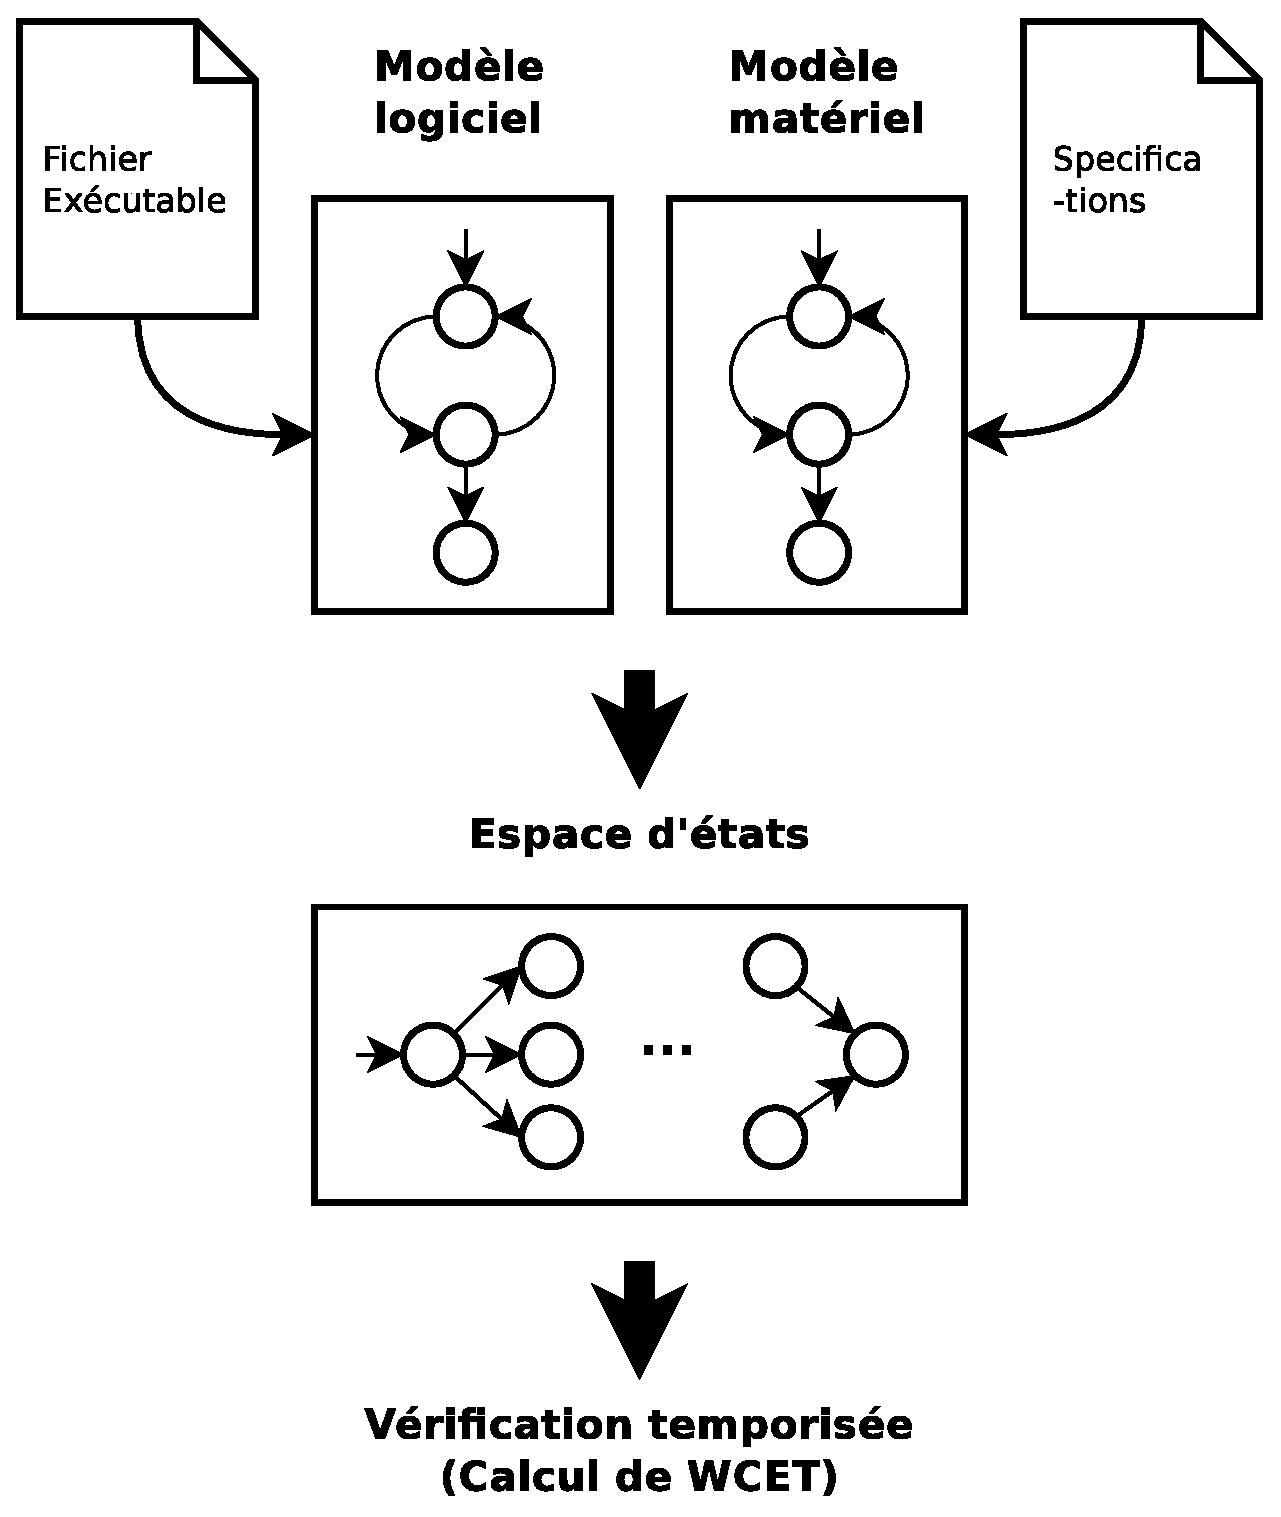
\includegraphics[scale=0.3]{intro.eps}
        \caption{Analyse temporelle par vérification de modèles temporisés}
        \label{fig:intro}
      \end{figure}

      \paragraph{Motivations}
      { Différentes approches d'analyse temporelle existent. Certaines se basent
        sur la prédiction des états du cache et du pipeline par interprétation
        abstraite et sur l'enumération implicite des chemins par optimisation
        linéaire en nombres entiers \cite{HF04}.

        Ces techniques définissent des algorithmes \textit{ad hoc}
        pour tenir compte des spécificités des architectures pour lesquelles le
        WCET est estimé. Un changement d'architecture implique donc
        l'écriture d'un nouvel algorithme. De plus, les résultats actuellement
        obtenus avec ces méthodes surestiment  les WCET réellement
        mesurés. Cela s'explique notamment par le fait que les modèles des
        équipements matériels utilisés font des abstractions nécessaires pour assurer la sûreté et la terminaison des calculs.

        Dans ces travaux, nous explorons une approche alternative basée sur l'analyse statique de modèles formels temporisés.

        \medskip
        
        Dans l'analyse temporelle basée sur les modèles formels temporisés,
        l'estimation du WCET s'obtient en explorant l'espace d'état du système
        résultant du produit synchronisé du modèle du programme et du modèle
        de l'architecture, comme le décrit la figure
        \ref{fig:intro}. Le calcul de WCET est donc réduit à un problème
        d'accessibilité, qui peut être résolu grâce aux méthodes de
        vérification de modèles temporisés existantes.

        Il existe différents outils de calcul de WCET à base de modèles formels
        temporisés~\cite{DOT10, CB13}. Leurs résultats expérimentaux montrent
        que cette approche permet de prendre en compte de façon détaillée
        l'architecture et d'ainsi obtenir des estimations de WCET sûres et
        précises. }
  
      \paragraph{Problèmatique}
      { 
        Il y a une dizaine d'année, il était reconnu par la communauté
        scientifique que les outils dee vérification de modèles temporisés
        n'offraient pas de performances suffisantes pour traiter le problème
        d'estimation du WCET~\cite{Wil04}.

        \medskip

        En dix ans, ces outils ont naturellement progressés, et profitent
        également des performances accrues des stations de travail. Cependant,
        le problème d'accessibilité reste complexe (PSPACE-complet pour les
        automates temporisés).
        Pour pallier ce problème, il paraît important de réduire au maximum la
        taille des modèles manipulés (en terme de nombre d'horloges et de nombre
        de localités).

        La technique que nous proposons d'employer pour réduire la taille des
        modèles de programme est le \textit{program slicing} sur les CFG
        reconstruits. Le \textit{slicing} d'un programme réduit celui-ci en un
        programme minimal reproduisant un comportement considéré
        \cite{Wei81}. Les comportements qui sont considérés ici sont ceux ayant
        trait au choix du chemin dans le graphe de flot de contrôle. }

%%%%%%%%%%%%%%%%%%%%%%%%%%%%%%%%%%%%%%%%%%%%%%%%%%%%%%%%%%%%%%%%%%%%%%%%%%%%%%%%
  
  \subsection{Approches existantes}
    \subsubsection{Reconstruction de CFG}
      \paragraph{Utilisation de fichiers sources en langage de haut-niveau}
      { Certaines méthodes de reconstruction des CFG de programmes s'appuient
        sur les fichiers sources en langage de haut-niveau des programmes
        considérés.

        Cependant, le comportement logiciel qui est effectivement constaté à
        l'exécution n'est pas strictement celui que definissent les fichiers
        sources de programmes en langage de haut-niveau. En effet, ces fichiers
        sources sont compilés vers des fichiers exécutables en langage de
        bas-niveau que la plateforme matérielle cible est en mesure
        d'exécuter.

        Par nature, il existe une différence d'expressivité entre les langages
        de haut et de bas-niveau. Lorsque cette différence n'est pas prise en
        compte lors de la reconstruction des CFG, les analyses temporelles
        réalisées sur la base de tels CFG sont imprécises.}%en sont d'autant imprécises. }
      
      \paragraph{Utilisation de connaissances sur les compilateurs}
      { Certaines méthodes de reconstruction des CFG se basant sur les fichiers
        exécutables des programmes s'appuient sur une connaissance des
        mécanismes internes des compilateurs.

        D'une part, cette connaissance n'est permise que par un travail
        fastidieux d'analyse des compilateurs. D'autre part, les mécanismes
        internes des compilateurs ne sont pas toujours librement accessibles. }

      \paragraph{Utilisation d'annotations}
      { Certaines méthodes de reconstruction des CFG proposent de réduire
        l'imprécision des CFG qu'elles produisent par leur annotation. Par
        exemple, lorsque le nombre maximal d'itérations d'une boucle ne peut
        être déterminé par la méthode employée, celui-ci peut être ajouté par
        annotation.
        
        De la même façon, ces méthodes dépendent d'un travail fastidieux étant,
        de plus, non sûr et non précis. }

      % FLP15: "Insight: An Open Binary Analysis Framework".

      \paragraph{L'outil \textsc{INSIGHT}}
      { Cet outil~\cite{FLP15} manipule des fichiers exécutables. Ceux-ci sont
        transposés dans une représentation intermédiaire sur laquelle peut être
        réalisée une analyse statique. Cette analyse est réalisée par une
        exécution symbolique de la représentation intermédiaire dans un domaine
        abstrait où chaque variable est substituée par une formule représentant
        toutes les valeurs possibles que celle-ci peut prendre. Cette exécution
        symbolique se base sur l'utilisation d'un solveur SMT.

        Une telle exécution permet la reconstruction de CFG. Cependant, cet
        outil, n'ayant pas été développé pour l'analyse des systèmes embarqués
        temps-réel, produit une sous-estimation du CFG réel par choix de
        conception. }

      % The00: "Extracting Safe and Precise Control Flow from Binaries".

      \paragraph{Approche ascendente}
      { Une autre approche~\cite{The00} définie une méthodologie ascendante de
          reconstruction de CFG. Celle-ci classifie chaque instruction du
          fichier exécutable considéré avant d'en réaliser une analyse. Un CFG
          interprocédural (ICFG) est défini en tant que la conjonction d'un
          graphe d'appel (CG) et d'un ensemble de CFG, à savoir un par
          sous-programme. Le CFG produit est construit en deux étapes. Un ICFG
          conservatif est tout d'abord construit à partir des informations que
          la classification des instructions permet d'obtenir. Ensuite une
          analyse statique basée sur la propagation de constantes est réalisée
          pour rafiner l'ICFG précédent. }
    
      % LS95: "EEL: Machine-Independent Executable Editing".
      %\cite{LS95}

      % CB13: "Timing Analysis of Binary Programs with UPPAAL".

      \paragraph{Approche par program slicing}
      { Une dernière approche~\cite{CB13} définit un processus reconstruction
        automatique de CFG à partir de fichiers exécutables. Cette génération
        est effectuée en deux étapes. La première reconstruit le CFG du
        programme par \textit{program slicing}. La seconde réduit le CFG
        également par \textit{program slicing}. }


%%%%%%%%%%%%%%%%%%%%%%%%%%%%%%%%%%%%%%%%%%%%%%%%%%%%%%%%%%%%%%%%%%%%%%%%%%%%%%%%

      %% Utilisation de la propagation de constante pour rafiner le CFG.

      \paragraph{Notre approche}
      { Notre approche est similaire à l'approche faisant usage du
          \textit{program slicing} évoquée plus haut. Elle ne s'appuie que sur
          les fichiers exécutables des programmes à analyser et ne nécessite
          donc ni les fichiers sources en langage de haut-niveau, ni l'ajout
          d'annotations.

        Notre approche ne fait pas non plus usage de connaissances sur les
        mécanismes des compilateurs. Grâce à l'outil \textsc{HARMLESS}
        \cite{KBB12} et à l'instar de la méthode ascendente décrite ci-dessus,
        nous procédons à une classification de chaque instruction avant
        d'effectivement procéder à la reconstruction du CFG.

        Enfin, à l'image de l'outil \textsc{INSIGHT} et une nouvelle fois grâce
        à l'outil \textsc{HARMLESS}, nous pouvons réaliser des simulations
        d'exécution. Ces simulations permettent la mise en {\oe}uvre de
        propagations de constantes utiles pour déterminer des plages de valeurs
        pour certains registres.

%%%%%%%%%%%%%%%%%%%%%%%%%%%%%%%%%%%%%%%%%%%%%%%%%%%%%%%%%%%%%%%%%%%%%%%%%%%%%%%%

    \subsubsection{Program slicing}
      \paragraph{L'approche arithmétique originale}
      { La définition originale du \textit{program slicing}~\cite{Wei81} est
        arithmétique. Elle fait usage d'un ensemble d'équations et d'un
        \textit{critère} pour déterminer quelles instructions font partie d'un
        \textit{slice}.

        Elle a été developpée pour s'appliquer sur des programmes structurés
        composés d'une unique procédure monolithique. On parle de
        \textit{slicing} intraprocédural. }

      \begin{figure}
        \centering
        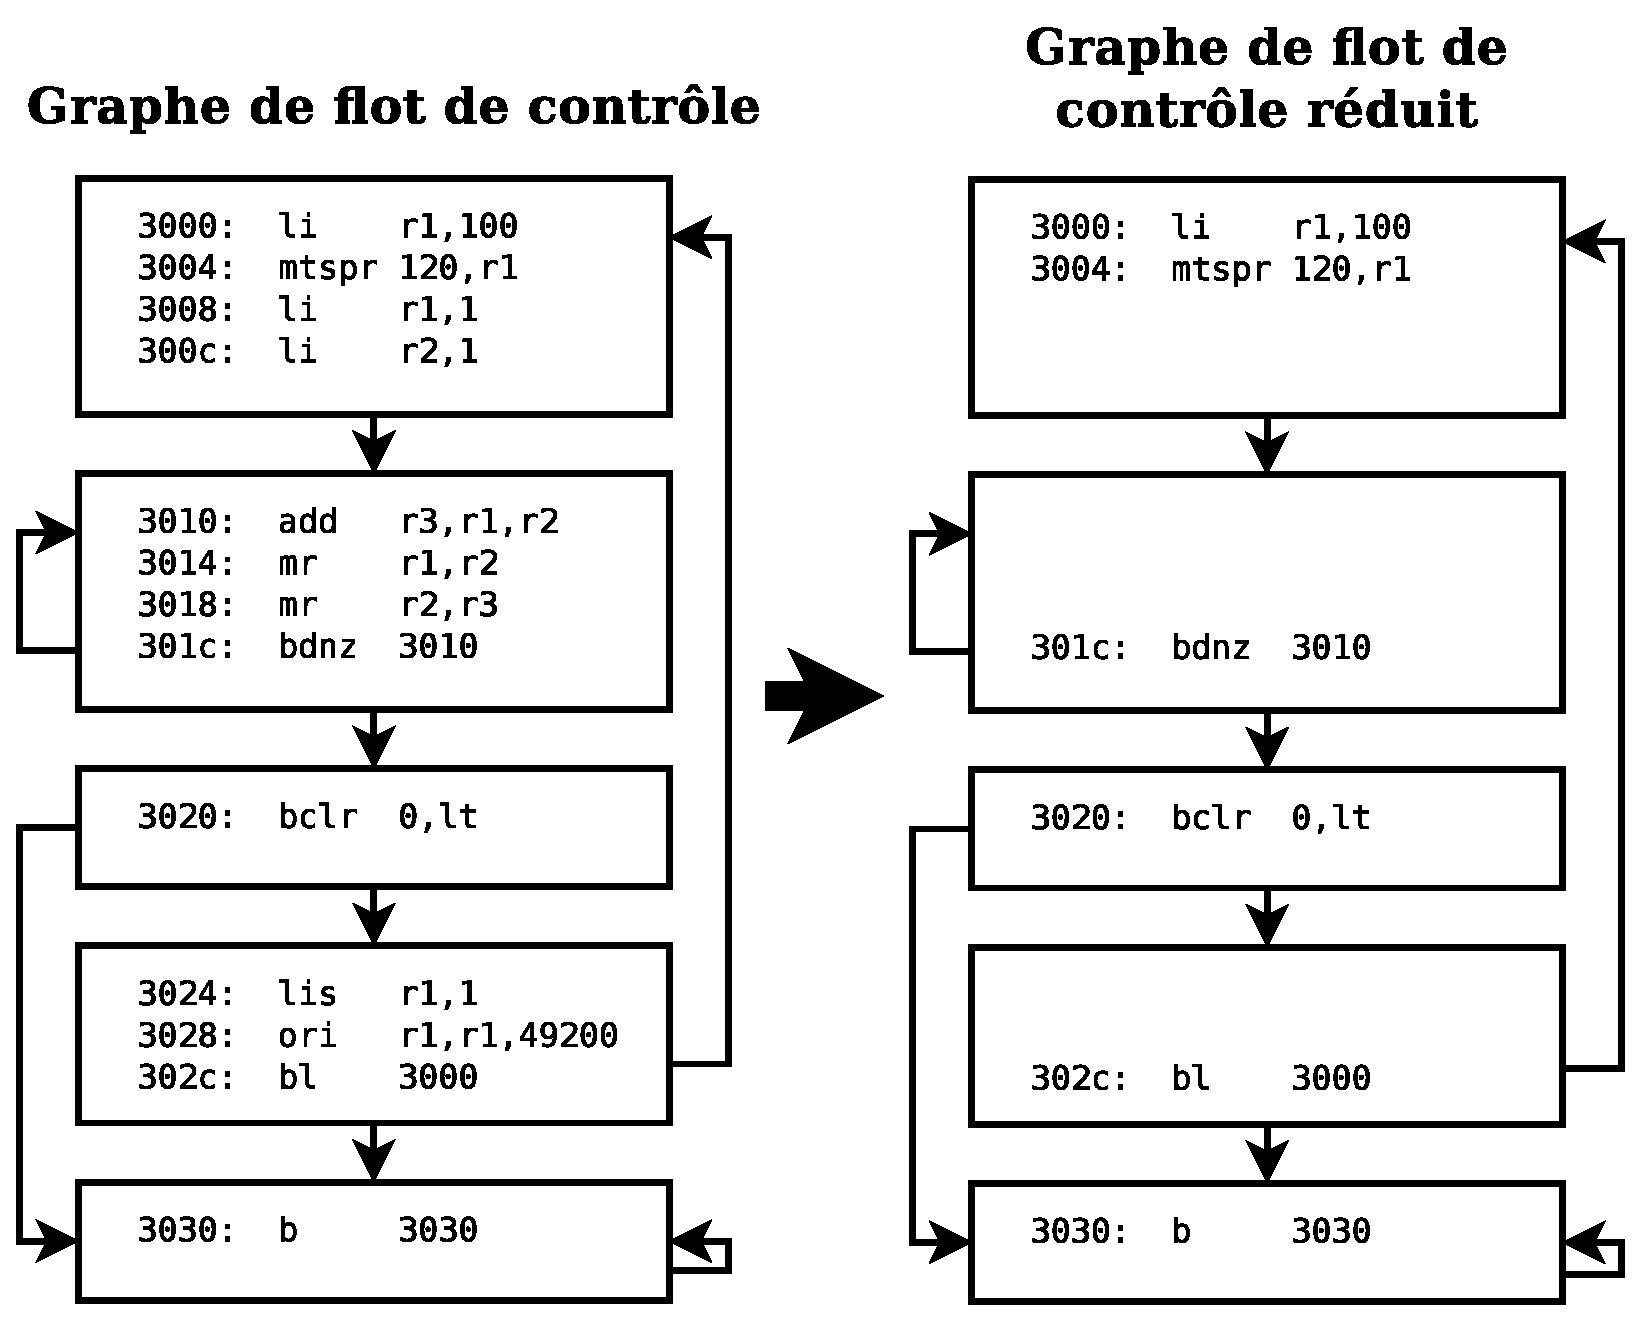
\includegraphics[scale=0.3]{slice.eps}
        \caption{Processus de réduction d'un CFG}
        \label{fig:slice}
      \end{figure}

      
      \paragraph{Les approches à base de graphe}
      { Lorsque le \textit{slicing} s'applique a un programme entier, tenant
        compte d'information obtenues au delà des frontières d'une procédure, on
        parle de \textit{slicing} interprocedural.

        Une autre définition du \textit{slicing} utilise une extension du
        concept de graphe de dépendance du programme (PDG) pour créer des
        \textit{slices} intraprocéduraux \cite{HRB90}. Cette méthode développe
        également le concept de graphe de dépendance du système (SDG) permettant
        la production de \textit{slices} interprocéduraux. Cette méthode permet
        de prendre en compte les contextes d'appel de chaque procédure.

        \medskip
        
        Des techniques similaires, intraprocédurales \cite{CF97} et
        interprocédurales \cite{KJL03}, ont été developpées pour fonctionner avec
        des programmes ayant des flots de contrôle arbitraires. Ces méthodes
        s'appuyent sur des graphes de dépendance de contrôle et de données
        spécialisés. }

      %% Pour ce faire un graphe de dépendance d'appel (CDG) est construit à
      %% partir d'un CFG et d'un graphe de dépendance de données (DDG)

      %% Une méthode aux résulats équivalents mais de mise en {\oe}uvre pratique
      %% plus simple a été développée \cite{Agr94}. Elle s'appuie sur l'arbre
      %% des postdominants, créé en paralèlle de la construction du SDG, ainsi
      %% qu'un arbre des successeurs lexicaux (LST).

      %% Une analyse statique intraprocédurale s'appuyant sur la méthode
      %% précédente a été développée \cite{CF97}. À la différence de cette
      %% dernière les dépendances de données du programme y sont représentées
      %% par des chaines de \textit{use-definition} plutôt qu'un DDG. Le slicing
      %% est réalisé en utilisant le CFG, le CDG, le PDT et les chaines de
      %% use-definition.
  
      %% Les sauts inconditionnels et les retours de fonctions sont ajoutés aux
      %% \textit{slices} et les labels de destinations des sauts sont
      %% determinés) d'un langage assembleur x86 simplifié (utilisant un CFG
      %% partiel ayant les blocs de base comme granularité) pour déterminer
      %% l'ensemble des instructions qui affectent les saut indirects.

      %% Une autre méthode définit un procédé pour construire un CFG
      %% interprocédural \cite{KJL03}. Les algorithmes de construction des CFG,
      %% CDG, DDG et PDG y sont modifiés ou étendus pour tenir compte des
      %% spécificités des fichiers exécutables. Une analyse de dépendance de
      %% contrôle et de données sont réalisées pour chaque fonction du CFG. Un
      %% CDG et un DDG sont construits suite à ces analyses ainsi qu'un PDG
      %% grâce aux CDGs et DDGs. Des \textit{slices} intraproceduraux peuvent
      %% être calculés en utilisant le PDG ainsi que des \textit{slices}
      %% interproceduraux en incorporant le PDG au SDG. C'est cette dernière
      %% méthode qui est utilisée.

      %% Utilisation d'outils de vérification d'automates temporisés
      %% \cite{LPY97} ou d'outils de vérification de réseaux de Petri temporels
      %% (ou de \textit{clock transition system} \cite{JLR14}) \cite{GLM05} pour
      %% l'analyse temporelle par vérification de modèle.  \medskip Le CFG ainsi
      %% reconstruit et réduit peut alors être exporté vers un format de
      %% représentation de modèles temporisés afin d'être vérifié par des outils
      %% de vérification temporisée.
